\chapter{Sistema de linealización}
\label{ch:linealizacion}

La corriente  $\ i_{pv} $ generada por un panel, posee un comportamiento exponencial, de manera que se requiere de una linealización.  Esta se realizará por medio de una función logarítmica que se estimará a través de un algoritmo de cálculo denominado CORDIC, el cual permite realizar una aproximación de la función de manera recursiva con una cantidad de iteraciones finita. El algoritmo de CORDIC para un logaritmo natural utiliza el sistema de coordenadas hiperbólico.

El rango de convergencia para este algoritmo es de $\ 0,106843 < T < 9,35947 $ donde $\ T $ es el argumento del logaritmo natural. El valor máximo $\ T = 0,58A $ es seleccionado a partir de la corriente en condiciones máximas para el panel. Para aprovechar de una mejor forma el intervalo de convergencia del algoritmo, se puede escalar por medio de una división entre una constante $\ C = 16$, esta es escogida de manera que se pueda realizar el escalado a través de desplazamientos. El nuevo intervalo de convergencia es limitado por: $\ 0.00667769 < T < 0.58496687 $. Este desplazamiento en el rango de convergencia  se realizó debido a que se pueden presentar valores de corriente mas bajos que 0.106843A.

La constante C utilizada en el escalado se debe compensar en el logaritmo con la siguiente igualdad: 

\begin{equation} \label{eq:ej1}
  Ln \left( T \right)
  = Ln \left( 16T \right) - Ln\left( 16 \right) 
\end{equation}  

  

\section{Algoritmo de CORDIC hiperbólico implementado en software}
 
Para comprobar el debido funcionamiento del este algoritmo se crea un programa de alto nivel en Python.  


\begin{figure}[H]
  \centering
    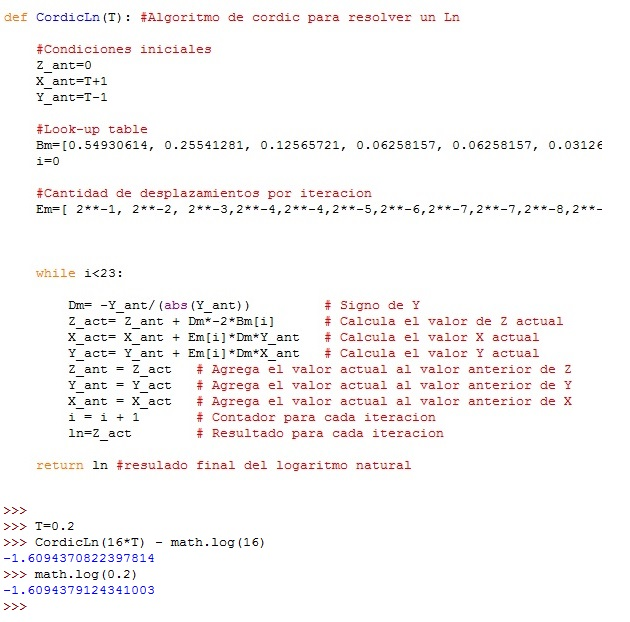
\includegraphics[scale=0.6]{./Progra_Cordic.jpg}
    \rule{35em}{0.5pt}
  \caption[Algoritmo de CORDIC en Python]{Algoritmo de CORDIC en Python  }
  \label{fig:Python}
\end{figure}


En la figura \ref{fig:Python} se observa el programa realizado para la verificación del algoritmo en alto nivel, para este se utilizan las ecuaciones para el algoritmo de CORDIC hiperbólico, descrito en el marco teórico. Este programa cuenta con las modificaciones realizadas en el rango de convergencia, con respecto al escalado y compensación. 

Para simplificar el diseño e implementación del hardware, se realiza una serie de modificaciones en las ecuaciones del algoritmo: 

\begin{compactitem}

\item Se sustituye la resta del valor actual de $ Z_{i+1} $ por una suma. 
\item Se incluye el signo en la tabla LUT de Z.
\item el resultado final del algoritmo se debe multiplicar por 2, sin embargo este escalado se puede realizar a los valores almacenados en la LUT de Z, esto para evitar una multiplicación. 
\end{compactitem}



\section{Sistema de linealización implementado en hardware (CORDIC)}

\begin{figure}[H]
  \centering
    \includegraphics[scale=0.06]{./Linealizador_general.png}
    \rule{35em}{0.5pt}
  \caption[Bloque principal de linealización: Entradas y salidas para la unidad logaritmo natural basada en el algoritmo de CORDIC e implementado en hardware]{Bloque principal de linealización: Entradas y salidas para la unidad logaritmo natural basada en el algoritmo de CORDIC e implementado en hardware. }
  \label{fig:CORDIC1}
\end{figure}

La figura \ref{fig:CORDIC1} contiene el bloque general del algoritmo de CORDIC, poseen 4 entradas: CLK , T , Begin\_LN , RST\_LN y 4 salidas: ACK\_LN , RESULT , U\_F , O\_F

\begin{figure}[H]
  \centering
    \includegraphics[scale=0.05]{./Linealizador_CORDIC_FSM.png}
    \rule{35em}{0.5pt}
  \caption[Sistema de linealización: Coprocesador coma flotante de 32bits basado en el algoritmo de CORDIC y una máquina de estados finita como control ]{Sistema de linealización: Coprocesador coma flotante de 32bits basado en el algoritmo de CORDIC y una máquina de estados finita como control.}
  \label{fig:CORDIC2}
\end{figure}

El sistema de linealización de la figura \ref{fig:CORDIC2} cuenta con dos módulos principales: 

\begin{compactitem}

\item \nt{Coprocesador Cordic}: Realiza todas las operaciones requeridas por el algoritmo, se encarga del manejo de los datos en el cálculo. 

\item \nt{Control}: Este se encarga de proveer las señales de control requeridas por el coprocesador, según las condiciones que se tenga en cada estado.

\end{compactitem}

Señales de datos: 

\begin{compactitem}

\item \nt{T}: Dato de entrada, argumento del logaritmo natural. 
\item \nt{RESULT}: Resultado de la operación logaritmo natural.

\end{compactitem}

Señales de control: 

\begin{compactitem}
\item \nt{CLK}: Reloj del sistema. 

\item \nt{Begin\_LN}: Encargada de dar inicio a la operación logaritmo natural. 

\item \nt{RST\_LN}: Realiza un reset a la unidad CORDIC tanto para el coprocesador como para la máquina de estados.
 

\item \nt{ACK\_LN}: Indica que el cálculo ya fue realizado.

\item \nt{Begin\_SUM}: Se encarga de dar inicio a la unidad de suma-resta coma flotante.

\item \nt{ACK\_SUM}: Indica que ha realizado el cálculo en la unidad de suma-resta coma flotante.

\item \nt{O\_F}: Indica si la suma-resta en coma flotante tiene un over-flow.

\item \nt{U\_F}: Indica si la suma-resta en coma flotante tiene un under-flow.

\item \nt{CLK\_DIR}: Activa el enable del contador de iteraciones. 

\item \nt{CONT\_ITER}: Indica el número de iteración y sirve de comparación para que la máquina de estados pueda detenerse en el número de iteraciones que se requieran.
 
\item \nt{RST}: Realiza el reset de todos los registros de la unidad.

\item \nt{MS\_1 , MS\_2 , MS\_3 , MS\_4}: Realizan la selección de cada multiplexor, Mux1, Mux2, Mux3, Mux's4 respectivamente.

\item \nt{EN\_REG1X , EN\_REG1Y , EN\_REG1Z}: Activa los enable de los registros de la primera etapa REG1X, REG1Y, REG1Z respectivamente, para almacenar datos. 

\item \nt{EN\_REG2XYZ}: Activa el enable del registro REG2XYZ de la segunda etapa. 

\item \nt{EN\_REG2}: Activa el enable del registro REG2 de la segunda etapa.

\item \nt{EN\_REG3}: Activa el enable del registro REG3 del dato inicial.

\item \nt{EN\_REG4}: Activa el enable del registro REG4 del dato final. 

\end{compactitem}

\section{Diseño e implementación del coprocesador de linealización por medio del algoritmo de CORDIC}
El diseño de este algoritmo se basa en una arquitectura segmentada, almacenando y procesando varios datos en las distintas etapas, para esto es de suma importancia una buena sincronización y así evitar datos erróneos a través del proceso de cálculo. Este coprocesador cuenta con el formato IEEE 754 de 32Bits, para una adecuada exactitud en la aproximación del logaritmo natural y poder utilizar un número menor de iteraciones.

\begin{figure}[H]
  \centering
    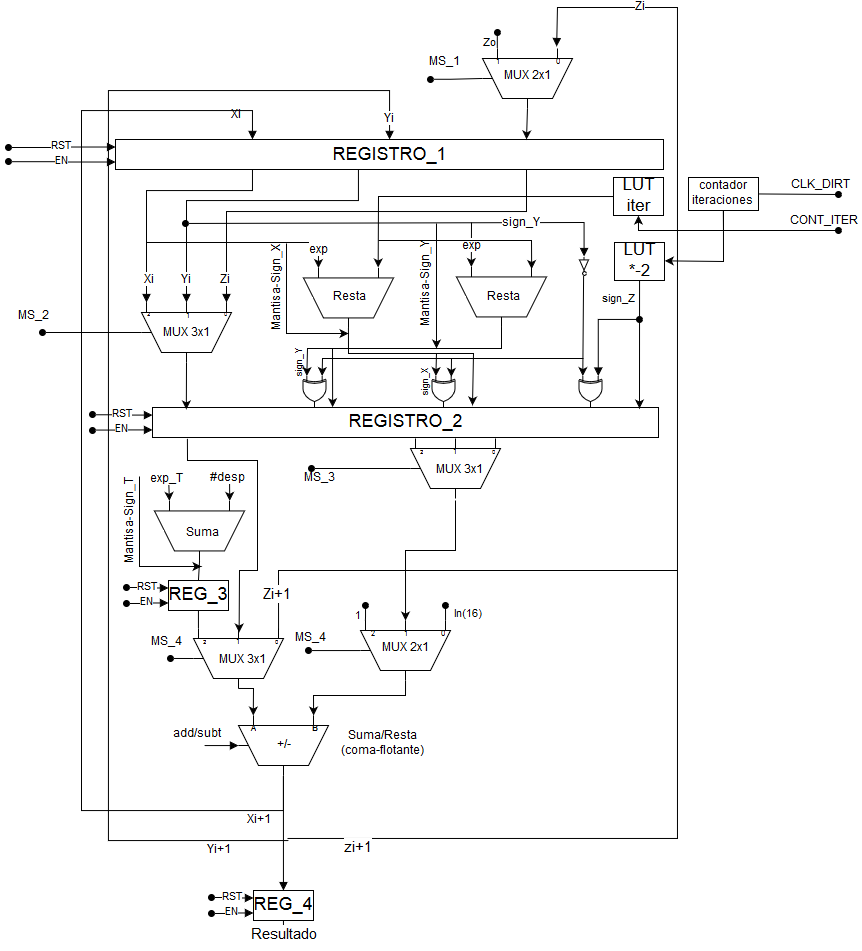
\includegraphics[scale=0.055]{./CORDICLN.png}
    \rule{35em}{0.5pt}
  \caption[Coprocesador segmentado para el cálculo de una función logarítmica con el algoritmo de CORDIC en hardware]{Coprocesador segmentado para el cálculo de una función logarítmica con el algoritmo de CORDIC en hardware  }
  \label{fig:CORDICLN}
\end{figure}
\newpage

En la figura \ref{fig:CORDICLN} se puede observar la arquitectura en formato IEEE 754 coma flotante en 32-Bits diseñada para el algoritmo de CORDIC.  

Esta etapa de linealización inicia con la carga de las condiciones iniciales, donde $\ Z_0 $ contiene un valor inicial cero. Para el valor inicial de $\ X_0 $ y $\ Y_0 $ primeramente se aplica el escalado  16*T, este se puede efectuar por medio de cuatro desplazamientos $\ 2^{-4} $, por lo tanto este movimiento en formato coma flotante, se traduce como una suma de 4 en el exponente del argumento $\ T$, posteriormente se realizan las siguientes operaciones en coma flotante,  $\ X_0 = T + 1 $ y $\ Y_0 = T - 1 $. Estas tres constantes dan inicio al proceso de cálculo de manera iterativa, por lo que se requiere almacenarlas en un registro $\ \left(Registro 1 \right) $ en la primera etapa de segmentación. 

Este método (CORDIC) es un cálculo cruzado es decir, para el próximo valor $\ X_i$ se requiere el valor de $\ Y_0 $ con un desplazamiento (resta en el exponente de la variable $\ Y_0 $)  y un cambio de signo $ \delta_i $. Para $\ Y_i $ se aplica un concepto similar con valores de $\ X_0$ según las ecuaciones que describen el algoritmo en modo hiperbólico. La variable de mayor interés es $\ Z_i $ esta contiene el valor final del cálculo, para esto se requiere una ROM con valores previamente cargados $\ \left(LUT_Z \right) $ y el signo $ \delta $.

Para el signo $ \delta $ de las operaciones en el algoritmo de CORDIC hiperbólico, se utiliza un circuito de comparación entre los signos de $\ X_i$,$\ Y_i$ y $\ Z_i$ contra el signo de $\ Y_i$ invertido, la siguiente tabla describe el funcionamiento del circuito diseñado: 

\begin{table}[H]
\centering
\caption{Signo $\ \delta $ de la iteración siguiente para las variables  $ X_{i+1} $ , $ Y_{i+1} $ y $ Z_{i+1} $, comparando el signo de las variables Xi , Yi y Zi contra el signo de Yi invertido}
\label{Table:Signo}
\begin{tabular}{|c|c|c|c|c|c|c|}
\hline
Sign $\ X_0 $ & Sign $\ Z_0 $  & Sign $\ Y_0 $ & Sign $\ \sim Y_0 $  & Sign $\ X_i $ & Sign $\ Z_i $  & Sign $\ Y_i $      \\ \hline

\begin{tabular}[c]{@{}c@{}} 0
\end{tabular}  & 0 & 0   & 1   & 1 & 1 & 1       \\ \hline

\begin{tabular}[c]{@{}c@{}} 0
\end{tabular} & 0 & 1   & 0  & 0 & 0 & 1       \\ \hline

\begin{tabular}[c]{@{}c@{}} 0 
\end{tabular} & 1 & 0   & 1 & 1 & 0 & 1\\ \hline
\begin{tabular}[c]{@{}l@{}} 0
\end{tabular} & 1 & 1   & 0  & 0 & 1 & 1   \\ \hline

\begin{tabular}[c]{@{}l@{}} 1
\end{tabular} & 0 & 0   & 1 & 0 & 1 & 1   \\ \hline

\begin{tabular}[c]{@{}l@{}} 1
\end{tabular} & 0 & 1   & 0  & 1 & 0 & 1   \\ \hline

\begin{tabular}[c]{@{}l@{}} 1
\end{tabular} & 1 & 0   & 1  & 0 & 0 & 1   \\ \hline

\begin{tabular}[c]{@{}l@{}} 1
\end{tabular} & 1 & 1   & 0 & 1 &  1 & 1    \\ \hline


\end{tabular}
\end{table}
\newpage


\begin{figure}[H]
  \centering
    \includegraphics[scale=0.06]{./signo.png}
    \rule{35em}{0.5pt}
  \caption[Circuito de comparación de signo actual $\ \delta$, para las variables $ X_{i+1} $ , $ Y_{i+1} $ y $ Z_{i+1} $ de la iteración siguiente, utilizando la tabla \ref{Table:Signo}]{Circuito de comparación de signo actual $\ \delta$, para las variables $ X_{i+1} $ , $ Y_{i+1} $ y $ Z_{i+1} $ de la iteración siguiente, utilizando la tabla \ref{Table:Signo}}
  \label{fig:SGN}
\end{figure}


A partir de la tabla \ref{Table:Signo} se extrae el circuito de comparación de signo de la figura \ref{fig:SGN}, este es diseñado con compuerta \nt{XOR} que poseen el mismo comportamiento que se describe en la tabla. 

Dentro del diseño del linealizador se requiere de tablas de rápido acceso, precargadas con los valores constantes para cada iteración. para esto se utilizan dos Look-up tables "LUT", que son diseñadas por medio de memorias ROM's, de manera que puedan ser accesados en cualquier momento que sean requeridos por medio de la dirección. 
Dentro de las ROM's se dispone:   

\begin{compactitem}

\item \nt{LUT\_Z}: Almacena los valores de $\ -2 \cdot arctanh \left( 2^{-i} \right) $, para cada iteración.  
\item \nt{LUT\_ITER}: Almacena los desplazamientos que se deben realizar para cada iteración, esto debido a que las iteraciones 4 y 13 repiten desplazamientos como se menciona en el marco teórico. 

\end{compactitem}


El acceso a cada valor de la tablas se realiza mediante un único contador de iteraciones, este indica a cada tabla la dirección del dato que se quiere extraer. Ambas LUT se encuentran sincronizadas en cuanto al numero de iteración. 

Anteriormente se describió el proceso para el cálculo de las constantes iniciales $ X_{0} $ , $ Y_{0} $ y $ Z_{0} $. El proceso para el cálculo de las variables $ X_{i+1} $ , $ Y_{i+1} $ y $ Z_{i+1} $, no se puede realizar de manera simultanea, ya que solo se cuenta con un sumador coma flotante, esta medida se tomó por reducción del área. 

Las variables modificadas (desplazamiento y signo) son almacenadas en el \nt{Registro 2}.
La secuencia de cálculo toma primeramente los valores que se necesitan para  $\ X_{i+1} $, posteriormente se realiza la suma $\ X_{i} +  \delta \cdot Y_{desplazado\_i} $ y se almacena el resultado en el \nt{Registro 1}. Seguidamente se procede con el cálculo de $\ Y_{i+1} $ y se realiza la suma $\ Y_{i} +  \delta \cdot X_{desplazado\_i} $ almacena en el \nt{Registro 1}, por ultimo se calcula el valor de $\ Z_{i+1} $, con la suma $\ Z_{i} +  LUT_i $, esta se almacena en el \nt{Registro 1}, este proceso se realiza N iteraciones (N=número entero). La resta  $\ Z_i - Ln\left(16\right) $ contrarresta el efecto del escalado aplicado al argumento $\ \left(T\right) $, al inicio del cálculo del logaritmo natural. El resultado final $\ Z_i $ contiene el valor $Ln \left(T \right)$ y es almacenado en el \nt{Registro 4}.

\section{Sistema de control para la unidad de coprocesamiento CORDIC por medio de un máquina de estados finita (FSM)}

\begin{figure}[H]
  \centering
    \includegraphics[scale=0.045]{./MaquinaL.png}
    \rule{35em}{0.5pt}
  \caption[Máquina de estados finitos para para la unidad de coprocesamiento CORDIC]{Máquina de estados finitos para para la unidad de coprocesamiento CORDIC}
  \label{fig:FSML}
\end{figure}

El sistema de control necesita mucha sincronía, ya que los datos deben ser almacenados de manera correcta y estar listos con cierto tiempo ("setup-time") antes de que requeridos por otro segmento del coprocesador CORDIC. Se diseñó una máquina de estados finitos, donde inicialmente se calculan los valores iniciales de $ X_0 $, $ Y_0 $ y $ Z_0 $, posteriormente la máquina brinda las señales de control requeridas, dentro de una secuencia de cálculo de $ X_{i+1} $,$ Y_{i+1} $ y $ Z_{i+1} $ respectivamente, cada vez que se recorre esta secuencia, se realizará una cuenta de iteración. Esa máquina posee con una variable de entrada que indica el número de iteración en el que se encuentra el algoritmo, de manera que cuando se llega a la iteración N, finalice el cálculo.

\section{Algoritmo de CORDIC implementado en verilog para una placa de desarrollo nexys-4}

Este algoritmo se implementó por medio del lenguaje de descripción de hardware "Verilog". Inicialmente se realizaron pequeños bloques pertenecientes a cada elemento requerido por la arquitectura diseñada. Se desarrolló el coprocesador CORDIC y la unidad de control en bloques separados, de manera que se pudieran realizar pruebas sin dependencia de los bloques entre si, para una mejor depuración de errores, optimización y rediseño. Finalmente se procede a la etapa de pruebas, con simulaciones al bloque completo, como se muestra en la figura \ref{fig:SIMLINEAL}. 

\begin{figure}[H]
  \centering
    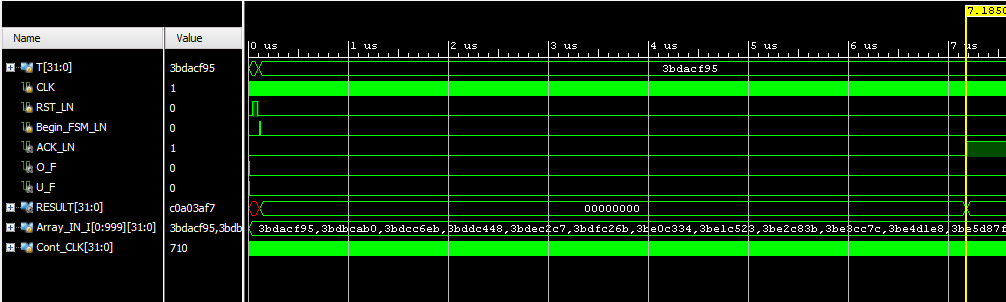
\includegraphics[scale=0.75]{./TEST_LINEALIZADOR_I.png}
    \rule{35em}{0.5pt}
  \caption[Simulación del linealizador implementado en Verilog, ingresando en la entrada un archivo de texto, con 1000 valores del intervalo de convergencia para el argumento del logaritmo natural]{Simulación del linealizador implementado en Verilog, ingresando en la entrada un archivo de texto, con 1000 valores del intervalo de convergencia para el argumento del logaritmo natural}
  \label{fig:SIMLINEAL}
\end{figure}   

\section{Simulación del circuito linealizador con algoritmo de CORDIC}

Las simulaciones de la implementación del algoritmo, se realizaron mediante mil valores de entrada para el argumento del logaritmo natural, dentro del rango de convergencia, obteniendo mil valores de salida. Estos resultados experimentales se comparan con los valores reales, para dicha comparación se realizaron aproximaciones con 8, 12 y 15 iteraciones. 

Primeramente se realiza una simulación que comprueba el funcionamiento en el rango de operación $\ 0,00667769 < T < 0,58496687 $. La linealización de los datos de prueba se realiza con la siguiente función: 

\begin{equation} \label{eq:ej2}
  Ln \left(T \right) 
\end{equation} 

donde el argumento T es:

\begin{equation} \label{eq:ej3}
   T = e^{-x}         
\end{equation} 
  
El intervalo $\ 0,536 < x < 5,009$ se divide en mil valores, estos se ingresan a la entrada por medio de un archivo de texto. El circuito linealizador CORDIC toma los datos, le aplica la función \ref{eq:ej2} y devuelve mil valores a través de otro archivo de texto, que se utilizará para análisis posteriormente. 
 

\subsection{Resultados de la simulación del rango de convergencia del circuito linealizador CORDIC}

Para implementar un algoritmo o método numérico en hardware, es de suma importancia verificar que este funcione de manera adecuada en el rango de convergencia definido. La comprobación de la unidad de linealización mediante el algoritmo de CORDIC, se realizó por medio de una serie de pruebas, variando la cantidad de iteraciones para poder observar las diferencias entre exactitud y tiempo de ejecución. Se programó una simulación ("testbench") con mil valores de entrada, ingresados por medio de un archivo de texto previamente editado con los datos de entrada, con la función exponencial anteriormente descrita en la ecuación \ref{eq:ej3}. 

En la tabla \ref{Table:comparacion_iter} se puede observar el resumen de los resultados más relevantes para las simulaciones del rango de convergencia con distinta cantidad de iteraciones del algoritmo de CORDIC. 

\begin{table}[H]
\centering
\caption{Comparación de resultados experimentales obtenidos por medio de una simulación post-síntesis, a partir de los valores de entrada del rango de convergencia, utilizando 8, 12 y 15 iteraciones en el algoritmo de CORDIC. CLK=100MHz. }
\label{Table:comparacion_iter}
\begin{tabular}{|c|c|c|c|c|c|c|}
\hline
$  $ & 8 iteraciones  & 12 iteraciones  & 15 iteraciones      \\ \hline

\begin{tabular}[c]{@{}c@{}} Error máximo (\%)
\end{tabular}  & 2,72 & 0,259   & 0,129         \\ \hline

\begin{tabular}[c]{@{}c@{}} Error promedio (\%)
\end{tabular}  & 0,40 & 0,0351   & 0,0257        \\ \hline

\begin{tabular}[c]{@{}c@{}} Desviación estándar 
\end{tabular} & 0,39 & 0,043   & 0,0197     \\ \hline

\begin{tabular}[c]{@{}c@{}} Número de ciclos 
\end{tabular}  & 460 & 660   & 818        \\ \hline

\begin{tabular}[c]{@{}c@{}} Frecuencia de ejecución (kHz) 
\end{tabular} & 217,39 & 151,51   & 122,25       \\ \hline

\begin{tabular}[c]{@{}l@{}} Tiempo de ejecución ($ \mu s$)
\end{tabular} & 4,6 & 6,6   & 8,18      \\ \hline


\end{tabular}
\end{table}

\begin{figure}[H]
  \centering
    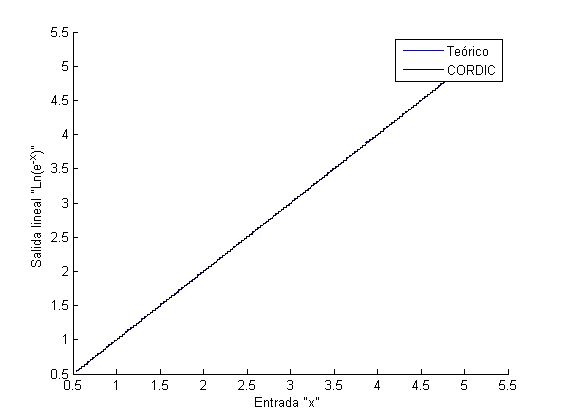
\includegraphics[scale=0.8]{./RANGO_8iter.png}
    \rule{35em}{0.5pt}
  \caption[Datos de salida para la simulación post-sintesis del linealizador, mediante mil valores de entrada dentro del rango de convergencia utilizando 8 iteraciones en el algoritmo de CORDIC]{Datos de salida para la simulación post-sintesis del linealizador, mediante mil valores de entrada dentro del rango de convergencia utilizando 8 iteraciones en el algoritmo de CORDIC }
  \label{fig:RG8}
\end{figure}

\newpage

\begin{figure}[H]
  \centering
    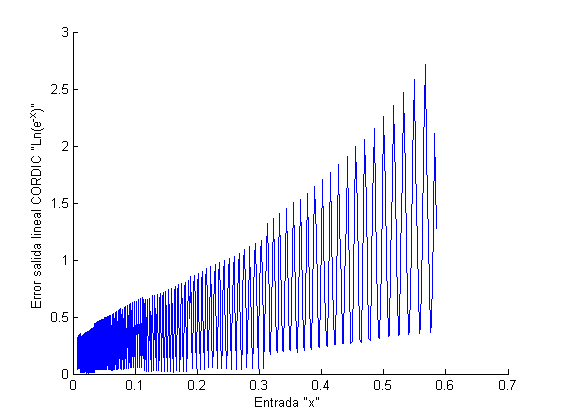
\includegraphics[scale=0.8]{./RANGO_8iter_ERROR.png}
    \rule{35em}{0.5pt}
  \caption[Porcentaje de error para los datos de la simulación post-síntesis del linealizador, tomando mil valores de entrada dentro del rango de convergencia y  8 iteraciones para el algoritmo de CORDIC]{Porcentaje de error para los datos de la simulación post-síntesis del linealizador, tomando mil valores de entrada dentro del rango de convergencia y  8 iteraciones para el algoritmo de CORDIC}
  \label{fig:RGE8}
\end{figure}


Primeramente se realizó una simulación con 8 iteraciones, en la figura \ref{fig:RG8} se muestran los valores obtenidos a partir de la simulación post-síntesis. Para el cálculo de cada valor se requieren 460 ciclos de reloj, desde el momento en se activa la señal Begin\_LN hasta que se recibe la señal ACK\_LN, esta indica que se ha completado el cálculo. Es de suma importancia realizar la comparación entre el valor teórico y el valor calculado. Para cada valor se calculó el error, la gráfica se puede observar en la figura \ref{fig:RGE8}, donde el porcentaje de error máximo es de 2,72\% y el porcentaje de error promedio es de 0,40\%. 

\newpage 
 
\begin{figure}[H]
  \centering
    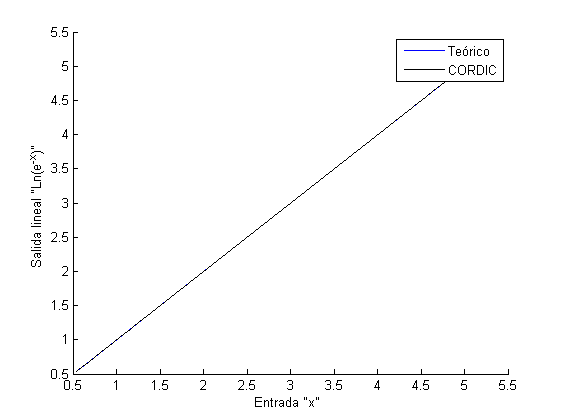
\includegraphics[scale=0.8]{./RANGO_12iter.png}
    \rule{35em}{0.5pt}
  \caption[Datos de salida para la simulación post-sintesis del linealizador, mediante mil valores de entrada dentro del rango de convergencia utilizando 12 iteraciones en el algoritmo de CORDIC]{Datos de salida para la simulación post-sintesis del linealizador, mediante mil valores de entrada dentro del rango de convergencia utilizando 12 iteraciones en el algoritmo de CORDIC}
  \label{fig:RG12}
\end{figure}

\begin{figure}[H]
  \centering
    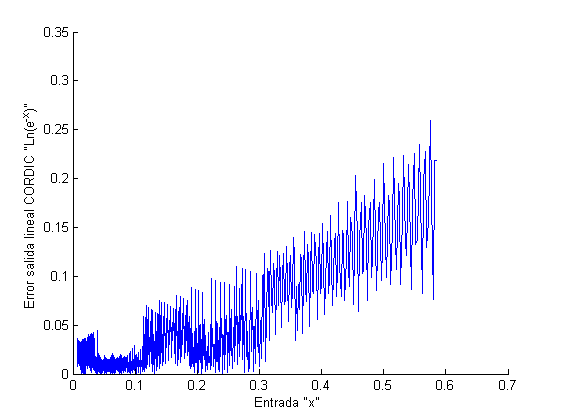
\includegraphics[scale=0.8]{./RANGO_12iter_ERROR.png}
    \rule{35em}{0.5pt}
  \caption[Porcentaje de error para los datos de la simulación post-síntesis del linealizador, tomando mil valores de entrada dentro del rango de convergencia y  12 iteraciones para el algoritmo de CORDIC]{Porcentaje de error para los datos de la simulación post-síntesis del linealizador, tomando mil valores de entrada dentro del rango de convergencia y  12 iteraciones para el algoritmo de CORDIC}
  \label{fig:RGE12}
\end{figure}

Una mejor aproximación se puede realizar utilizando 12 iteraciones en el cálculo del logaritmo natural, en la figura \ref{fig:RG12} se pueden observar los resultados obtenidos. Se requieren 660 ciclos de reloj para ejecutar el cálculo completo. La figura \ref{fig:RGE12} muestra el error en cada cálculo, donde el porcentaje de error máximo es de  0,259\% y el porcentaje de error promedio es de 0,0351\%. 

\begin{figure}[H]
  \centering
    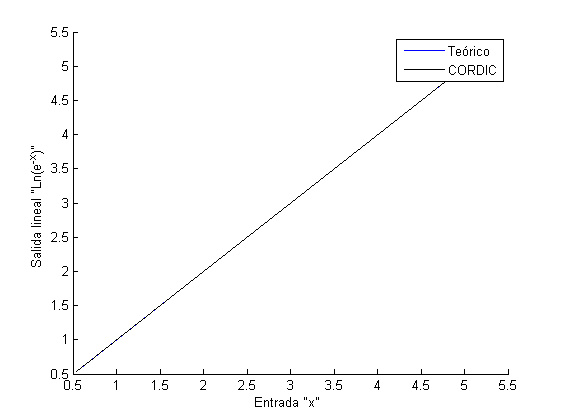
\includegraphics[scale=0.8]{./RANGO_15iter.png}
    \rule{35em}{0.5pt}
  \caption[Datos de salida para la simulación post-sintesis del linealizador, mediante mil valores de entrada dentro del rango de convergencia utilizando 15 iteraciones en el algoritmo de CORDIC]{Datos de salida para la simulación post-sintesis del linealizador, mediante mil valores de entrada dentro del rango de convergencia utilizando 15 iteraciones en el algoritmo de CORDIC}
  \label{fig:RG15}
\end{figure}

\newpage

\begin{figure}[H]
  \centering
    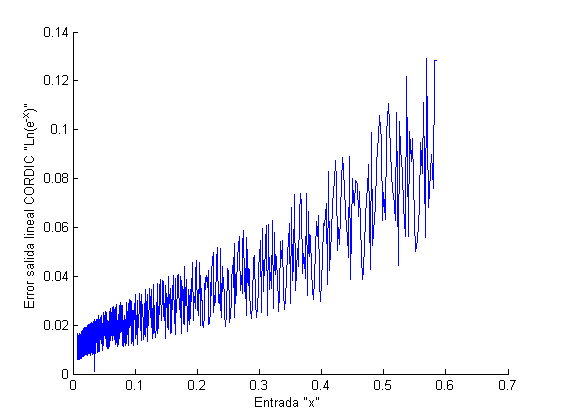
\includegraphics[scale=0.8]{./RANGO_15iter_ERROR.png}
    \rule{35em}{0.5pt}
  \caption[Porcentaje de error para los datos de la simulación post-síntesis del linealizador, tomando mil valores de entrada dentro del rango de convergencia y  8 iteraciones para el algoritmo de CORDIC]{Porcentaje de error para los datos de la simulación post-síntesis del linealizador, tomando mil valores de entrada dentro del rango de convergencia y  8 iteraciones para el algoritmo de CORDIC}
  \label{fig:RGE15}
\end{figure}


Utilizando 15 iteraciones en el cálculo del logaritmo natural se logra la mejor aproximación, sin embargo se requieren 818 ciclos de reloj y se vuelve más lento el proceso, en la figura \ref{fig:RG15} se pueden observar los resultados obtenidos. La figura \ref{fig:RGE15} muestra el error en cada cálculo, donde el porcentaje de error máximo es de  0,129\% y el porcentaje de error promedio es de 0,0257\%. 


En las figuras de error \ref{fig:RGE8}, \ref{fig:RGE12} y \ref{fig:RGE15} se puede observar que el comportamiento del algoritmo es más exacto cuando los valores de corriente de entrada del argumento de linealizador "T" son pequeños, a medida que este argumento se vuelve mayor el porcentaje de error también incrementa. 